% -------------------------------------------------
\section{Methods and Materials}\label{sec:methods}
% -------------------------------------------------

\subsection{System Architecture}\label{subsec:architecture}
Figure~\ref{fig:architecture} summarises the pipeline.  
A \textbf{Python Ingestor} polls the \textit{AQICN} download endpoint, the \textit{Google Air Quality API}, and the \textit{IQAir API} every ten minutes, saving raw JSON to a versioned MinIO bucket (\texttt{raw-airquality}) for replay and audit purposes\cite{minio,aqicnhist,googleair,iqair}.  
A stateless \textbf{Normalizer} aligns field names, units, and AQI scales before inserting each record into a TimescaleDB hypertable partitioned by \textit{month} and \textit{city}\cite{timescale}.  
Query acceleration relies on concurrent materialised views refreshed with \texttt{REFRESH MATERIALIZED VIEW CONCURRENTLY}\cite{postgsmv}.  
Read-heavy traffic is served from two hot stand-by replicas; Grafana dashboards visualise ingest lag, API latency, and view-refresh duration in real time\cite{grafana}.  

\begin{figure}[tb]
  \centering
  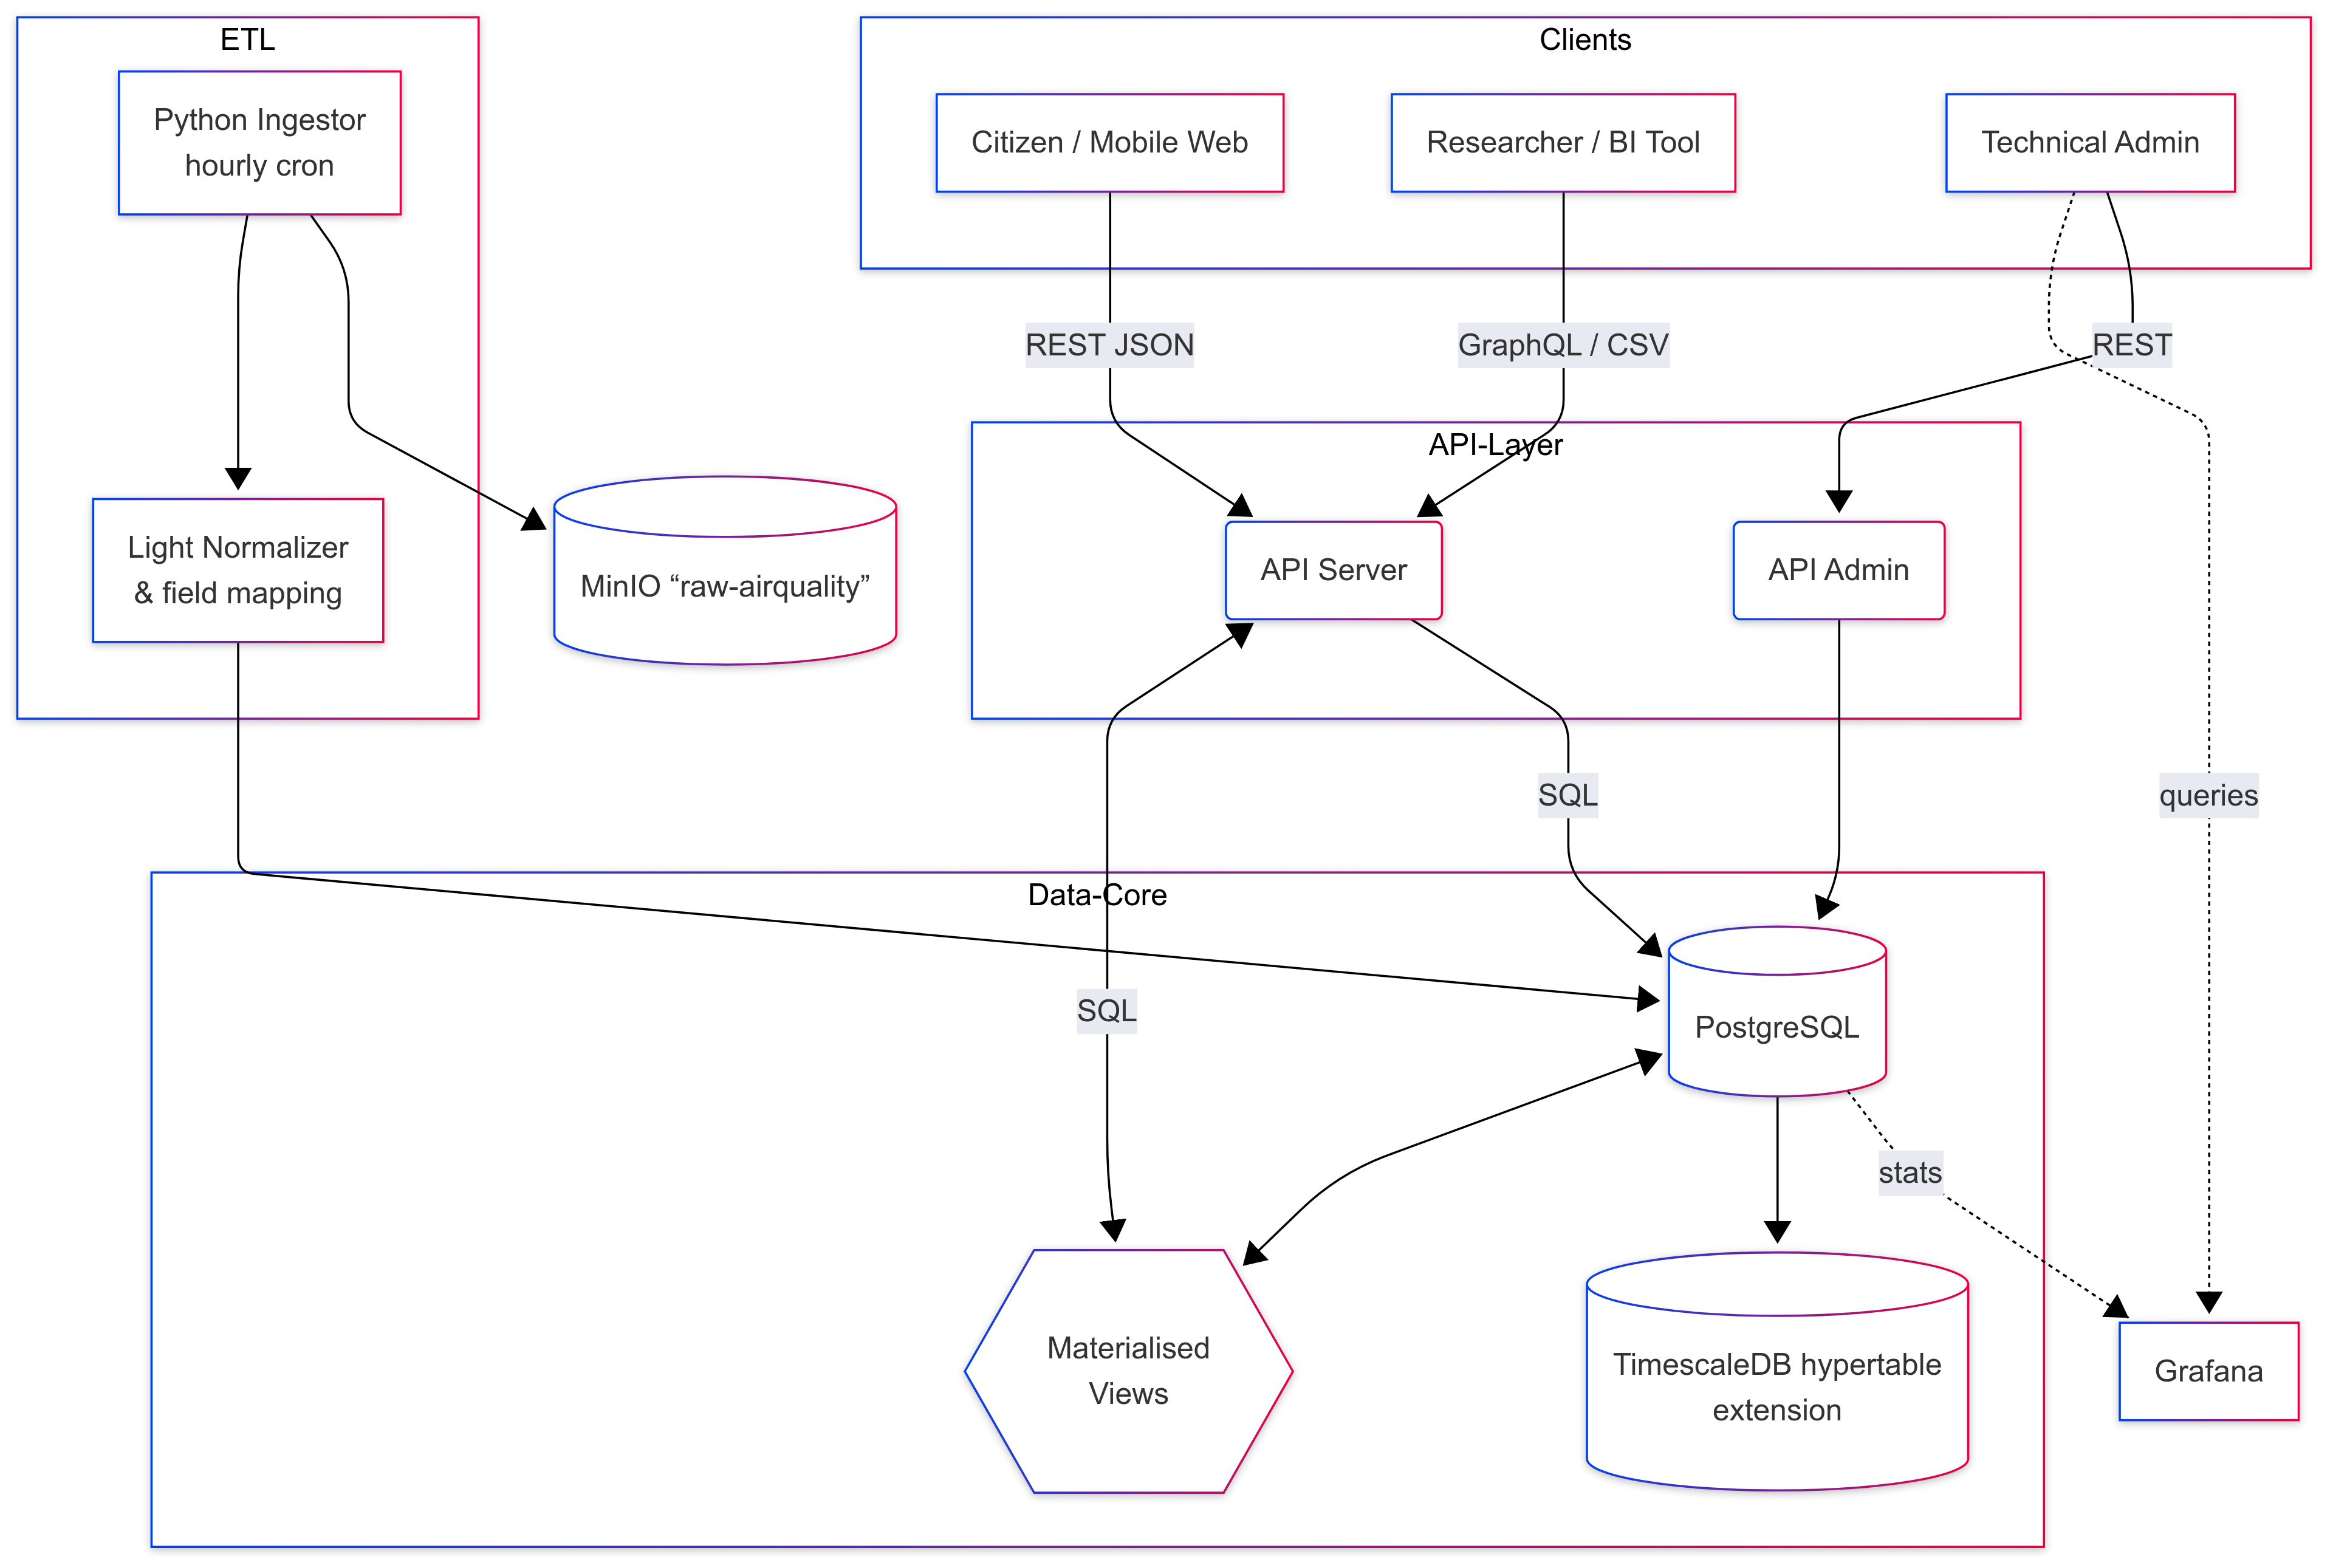
\includegraphics[width=\linewidth]{Pictures/fig1_architecture.png}
  \caption{End-to-end architecture (planned).}
  \label{fig:architecture}
\end{figure}

\subsection{Data Modelling and Partitioning}\label{subsec:partitioning}
The primary table \texttt{airquality\_reading} is a monthly-partitioned hypertable whose chunks never exceed \(\approx\!2.5\;\mathrm{M}\) rows for Bogotá (worst case)\cite{timescale}.  
Foreign keys link station metadata, pollutant codes, and regional polygons defined in the ER diagram.  
Prototype DDL and index configuration scripts are available in the project repository (omitted here for space).

\subsection{Personalised Recommendation Engine}\label{subsec:reco}
A rule-based service classifies every new observation into EPA AQI bands\cite{epaaqi}; combines that class with the user’s risk profile and intended activity; injects WHO health-advice snippets\cite{whoaq}; and optionally appends product suggestions when \(\text{AQI}\ge151\).  
Recommendations are cached in RAM (LRU, 3-hour TTL) to prevent redundant notifications during stable pollution periods.

\subsection{Planned Experimental Environment}\label{subsec:experiment}
Because the platform is still under active construction, we specify the \textit{target} test bench so reviewers can reproduce forthcoming benchmarks:

\begin{itemize}
  \item \textbf{Dataset.} Historical CSV archives published by AQICN starting in 2015\cite{aqicnhist}.  
        For phase 1 we will ingest the most recent three years (2022–2024) of Bogotá data; phase 2 expands to 2018–2024 if storage and ingest latency remain within budget.
        Each CSV row follows the schema
        \texttt{Date,Country,City, Specie,count,min, max,median,variance}.
  \item \textbf{Hardware (planned).} Primary DB node: 4 vCPU, 16 GB RAM, NVMe 500 GB; two identical read replicas; MinIO on a 4 TB RAID-1 array.
  \item \textbf{Software versions (expected).} PostgreSQL 17.1, TimescaleDB 2.14, MinIO 2025-06-13, Grafana 11, Python 3.12.
  \item \textbf{Load test design.} An Apache JMeter script will emulate 1 000 concurrent dashboard users, each issuing 5 REST requests s⁻¹ for 10 min\cite{jmeter}.  
        Prometheus exporters plus \texttt{pg\_stat\_statements} feed latency and resource metrics to Grafana\cite{grafana}.
\end{itemize}